% \newpage
% \section{Database design}

This project uses Firebase Cloud Firestore as a database. It is a NoSQL, document-oriented database. Unlike a SQL database, there are no tables or rows, instead, the data is stored in documents, which are organized into collections.

Each document contains a set of key-value pairs. Cloud Firestore is optimized for storing large collections of small documents. All documents must be stored in collections. Documents can contain subcollections and nested objects, both of which can include primitive fields like strings or complex objects like lists. \cite{firebase-datamodel}

The point of using Firebase is that it makes reading and writing very easy directly from the client app and you don't have to deal with any server configuration. The standard for a project like this one is to have a server with a SQL database installed, code a middle-ware that exposes the data through a REST API, and access the data from the client. But all these steps require a lot of time. And with Firebase you just access the data from the client. Firebase makes it exaggeratedly fast setup, simple to scale, and easy to maintain. 

\vfill
\begin{figure}[ht!]
    \center
    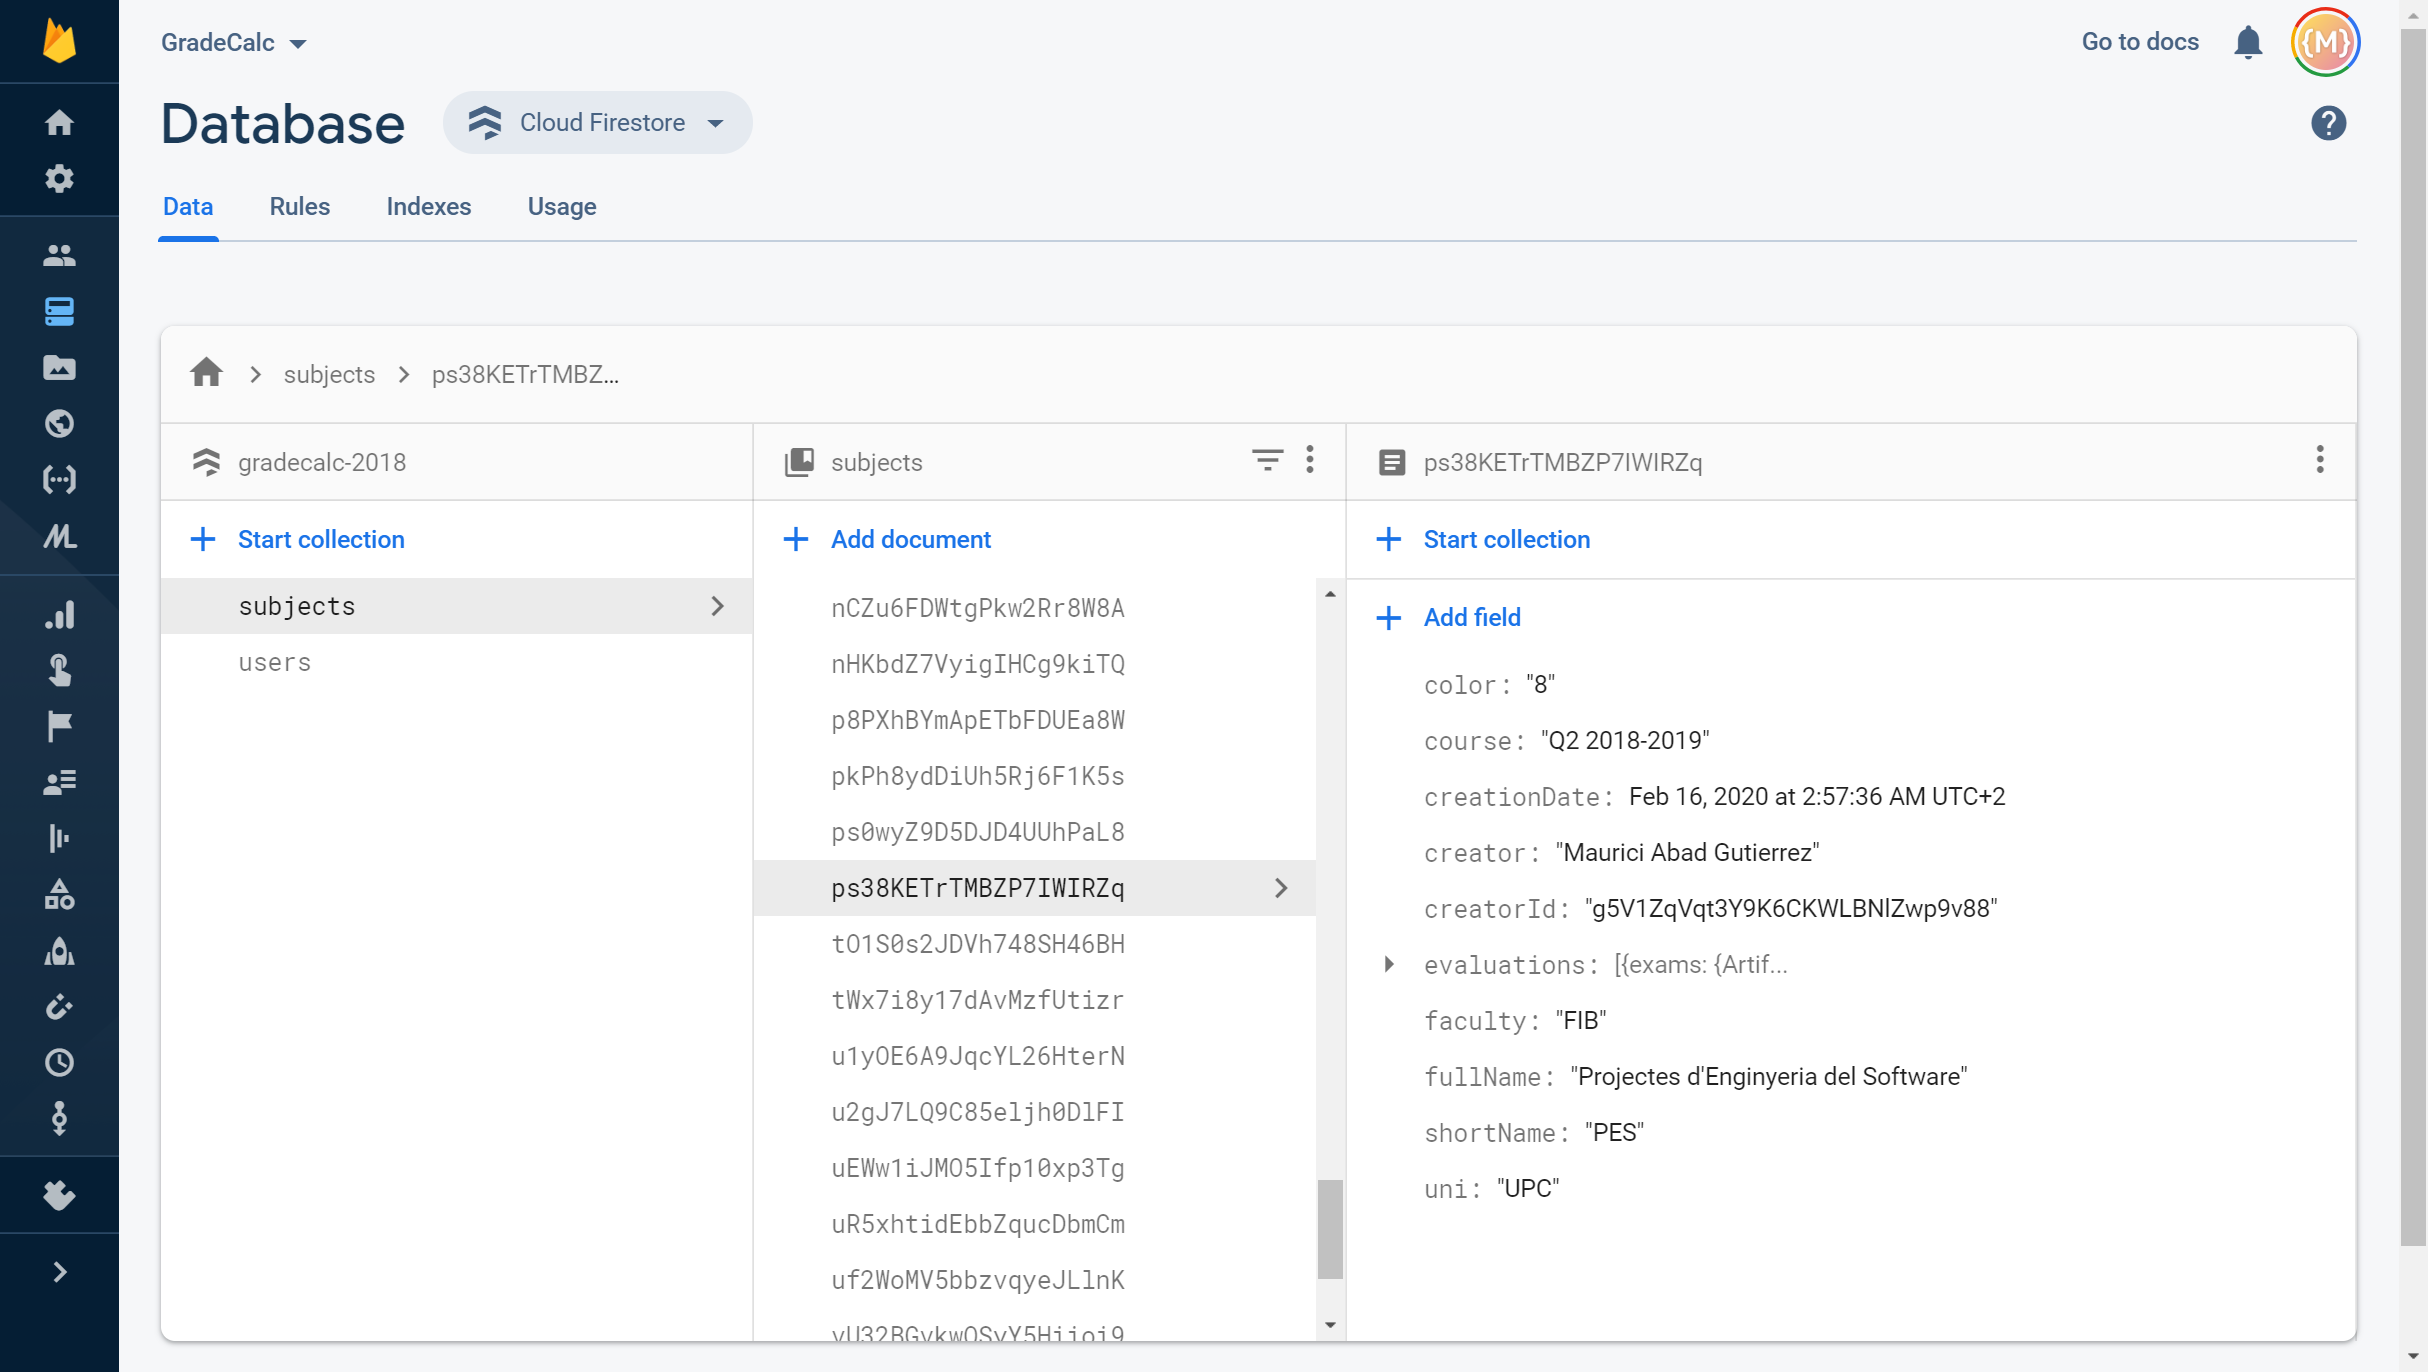
\includegraphics[width=0.9\textwidth]{media/firebase-console.png}
    \caption{Screenshot of Firebase Console}
    \label{fig:firebase-console}
\end{figure}
\vfill

\clearpage\newpage
\subsection{Data model}
\label{sec:data-model}

% \subsection{Data model in TypeScript for Firebase}
The firebase database has two collections, users and subjects, that contain \texttt{User} and \texttt{Subject} objects respectively. The database is defined in TypeScript, so this is its definition in TypeScript.

The attributes \texttt{Evaluation.name} and \texttt{Exam.name} must be unique in the array. The attribute \texttt{Exam.grade} can be undefined when the user hasn't done the exam. And, the attribute \texttt{Evaluation.selected} can be undefined when the subject is not assigned to a user.

% \subsubsection{User}
% \label{sec:user-data-model}
\vfill
\begin{minted}[
    baselinestretch=1,
]{typescript}
interface User {
  subjects: Array<Subject>
}
\end{minted}

\vfill

% \subsubsection{Subject}
% \label{sec:subject-data-model}

\begin{minted}[
    baselinestretch=1,
]{typescript}
interface Subject {
  color: number,
  course: string,
  creationDate: Date,
  creator: string,
  creatorId: string,
  evaluations: Array<Evaluation>,
  faculty: string,
  fullName: string,
  shortName: string,
  uni: string,
}

interface Evaluation {
  name: string,
  selected?: boolean,
  exams: Array<Exam>
}

interface Exam {
  name: string,
  type: string,
  weight: number,
  grade?: number
}
\end{minted}


\clearpage\newpage\noindent
% \subsubsection{Data model in UML}
For a clearer explanation, here is a UML diagram for the database. Although TypeScript represents it better. % noSQL is difficult to represent with UML

\vfill
\begin{figure}[ht!]
    \center
    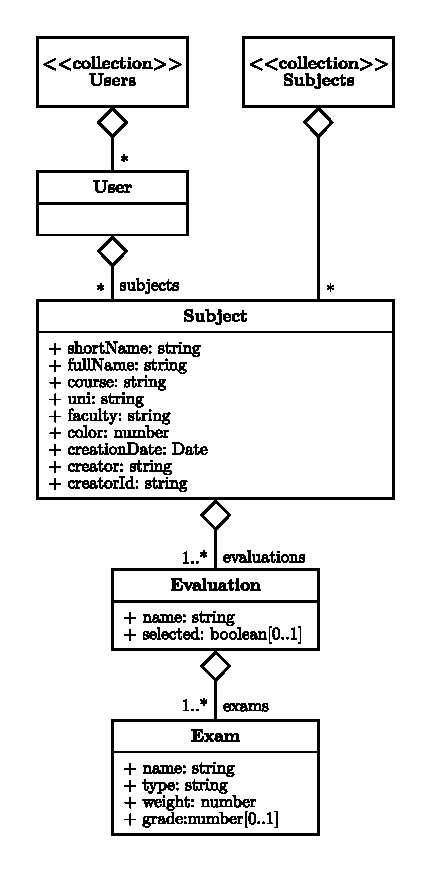
\includegraphics[height=19.5cm]{media/diagrams/database-uml.pdf}
    \caption{Data model's UML Diagram}
    \label{updated-gantt}
\end{figure}
\vfill
% textual restrictions: 0 <= weight <= 1

\clearpage\newpage
\subsection{Example objects}

These examples will help in understanding the object's structure.

\subsubsection{Example of a subject}

This is an example of a subject, in the subjects collection. It has basic information like \texttt{shortName}, \texttt{fullName} or \texttt{course}, and also two evaluations. Each evaluation has exams that have a \texttt{name}, \texttt{weight} and \texttt{type}. Notice that some exams are in both evaluations, this means that they represent the same available item but can be weighted different in each evaluation.

\vfill
\begin{minted}[
    baselinestretch=1,
]{typescript}
{
  shortName: "EDA",
  fullName: "Estructures de Dades i Algorismes",
  course: "Q2 2019-2020",
  uni: "UPC",
  faculty: "FIB",
  color: 2,
  evaluations: [
    {
      name: "Continua",
      exams: [
        { name: "P1",  weight: 0.3, type: "Exàmens" },
        { name: "PC",  weight: 0.3, type: "Exàmens" }
        { name: "F",   weight: 0.3, type: "Exàmens" },
        { name: "Joc", weight: 0.2, type: "Joc" }
      ]
    }, {
      name: "Final",
      exams: [
        { name: "PC",  weight: 0.3, type: "Exàmens" },
        { name: "F",   weight: 0.6, type: "Exàmens" },
        { name: "Joc", weight: 0.2, type: "Joc" }
      ]
    }
  ],
  creationDate: "February 28, 2020 at 9:39:50 PM UTC+1",
  creator: "Maurici Abad Gutierrez",
  creatorId: "4wUPZqVqt1Y9K6CAWLBNlZwe3b12"
}
\end{minted}
\vfill

\newpage
\subsubsection{Example of a user}
This user has only one subject saved. He changed its color (from color 2 to color 7) and saved some grades (8.33 in P1 and 5.5 in PC). Notice that because he hasn't done the exam "Joc", it's not stored. Also, he has the \textit{Continua} evaluation selected and changed the \texttt{color}. 

The subject's entire information is duplicated because if the original subject is edited, the data inside the user doesn't change, to prevent unexpected changes.

This object structure is optimized for NoSQL databases because it contains all the information needed to load the screen.

\vfill
\begin{minted}[
    baselinestretch=0.85,
]{typescript}
{
  subjects: [
    {
      shortName: "EDA",
      fullName: "Estructures de Dades i Algorismes",
      course: "Q2 2019-2020",
      uni: "UPC",
      faculty: "FIB",
      color: 7,
      evaluations: [
        {
          name: "Continua",
          selected: true,
          exams: [
            { name: "P1",  weight: 0.3, type: "Exàmens", grade: 8.33 },
            { name: "PC",  weight: 0.3, type: "Exàmens", grade: 5.5 }
            { name: "F",   weight: 0.3, type: "Exàmens" },
            { name: "Joc", weight: 0.2, type: "Joc" }
          ]
        }, {
          name: "Final",
          selected: false,
          exams: [
            { name: "PC",  weight: 0.3, type: "Exàmens", grade: 5.5 },
            { name: "F",   weight: 0.6, type: "Exàmens" },
            { name: "Joc", weight: 0.2, type: "Joc" }
          ]
        }
      ],
      creationDate: "February 28, 2020 at 9:39:50 PM UTC+1",
      creator: "Maurici Abad Gutierrez",
      creatorId: "4wUPZqVqt1Y9K6CAWLBNlZwe3b12"
    }
  ]
}
\end{minted}
\vfill
